% -*- coding: utf-8 -*-
% !TEX program = xelatex
%---------------------------------------------------------------------------
%         _                                     _   _               _     
%   _   _| | __     ___ _ __  _ __  _   _      | |_| |__   ___  ___(_)___ 
%  | | | | |/ /____/ __| '_ \| '_ \| | | |_____| __| '_ \ / _ \/ __| / __|
%  | |_| |   <_____\__ \ | | | | | | |_| |_____| |_| | | |  __/\__ \ \__ \
%   \__, |_|\_\    |___/_| |_|_| |_|\__,_|      \__|_| |_|\___||___/_|___/
%   |___/                                                                 
%---------------------------------------------------------------------------
%     模板名称 : yk-snnu-thesis
%     模板功能 : 陕师大博士/硕士论文模板
%     模板用法 : 
%               1. 复杂编译 : xelatex + biber + 3*xelatex  
%               2. 简单编译 : latexmk -xelatex
%     最近更新 : 2022年3月27日
%     作者信息 : 杨玉坤,陕西师范大学,物理学院,原子与分子物理
%     联系方式 : yykphy@gmail.com ; yk@snnu.edu.cn ; yangyukun@htu.edu.cn 
%     注意事项 :
%               1. 使用本模板,需致谢本模板或作者。
%               2. 本模板不是官方模板,一切后果自负。
%               3. 如果您有不同意见,那么您是对的,我是错的。
%---------------------------------------------------------------------------

\documentclass[twoside, 12pt, openright, no-math, AutoFakeBold]{ctexbook}
\usepackage{yk}


\begin{document}
    \frontmatter
        \pagestyle{empty}
            % -*- coding: utf-8 -*-
% !TEX program = xelatex

%==================================================
%=======           填写个人信息
%==================================================
\newcommand\clcNumber{O123}
\newcommand\securityClassification{公开}
\newcommand\studentId{B12345}
\newcommand\thesisTitleCN{陕西师范大学博士论文\LaTeX 模板}
\newcommand\thesisTitleEN{PhD thesis \LaTeX \; template of Shaanxi Normal University }
\newcommand\thesisAuthor{杨玉坤}
\newcommand\supervisor{张松斌 \quad 教授}
\newcommand\subjectFirst{物理学}
\newcommand\subjectSecond{原子与分子物理}
\newcommand\subdate{二〇二二年五月}




%==================================================
%=======               设置封面
%=======   不建议改动以下内容,除非你懂自己在做什么
%==================================================
{
    \setlength\parindent{0em}                                                 % 设置缩进
    \renewcommand{\baselinestretch}{2}\selectfont                             % 设置行间距
    % \ThisTileWallPaper{\paperwidth}{\paperheight}{pic/snnu/bgold.jpg} % 设置封面背景
    \ThisTileWallPaper{\paperwidth}{\paperheight}{pic/snnu/bgnew.pdf}    % 设置封面背景
    \vspace*{-3.0cm}
    {
        \zihao{-3}
        \begin{tabular}{l@{}c p{3cm} l@{}c}
            \heiti{分\ 类\ 号}    \quad      & \underline{\makebox[3cm][c]{\clcNumber}} \\
            \heiti{密\quad \ \ 级}\quad      & \underline{\makebox[3cm][c]{\kaishu \securityClassification}} \\
            \heiti{学\quad \ \ 号}\quad      & \underline{\makebox[3cm][c]{\studentId}} \\
        \end{tabular}
    } \par
    \vspace{8.5cm}
    \begin{center}
        \begin{tabular}{rc}
            \zihao{-3} \heiti {\bfseries 题\quad 目} & \UnderlineCentered{13cm}{1.5mm}{\zihao{-3} \heiti \thesisTitleCN \\ \thesisTitleEN}\\
        \end{tabular}
    \end{center}
    \vspace{1.5cm}
    {
    \newlength{\yklength}
    \setlength{\yklength}{\widthof{一二三四五六七八九}}
    \begin{center}
    \begin{tblr}{colspec = {Q[c, m, \yklength]Q[c, t, 13\ccwd]},}
        {\zihao{-3} \heiti 作\hfill 者 }                                    & \CJKunderline[thickness=0.6pt]{\makebox[14\ccwd]{\zihao{-3}\kaishu\thesisAuthor}} \\
        {\zihao{-3} \heiti 指\hfill 导\hfill 教\hfill 师}                   & \CJKunderline[thickness=0.6pt]{\makebox[14\ccwd]{\zihao{-3}\kaishu\supervisor}} \\
        {\zihao{-3} \heiti 一\hfill 级\hfill 学\hfill 科\hfill 名\hfill 称}  & \CJKunderline[thickness=0.6pt]{\makebox[14\ccwd]{\zihao{-3}\kaishu\subjectFirst}} \\
        {\zihao{-3} \heiti 二\hfill 级\hfill 学\hfill 科\hfill 名\hfill 称}  & \CJKunderline[thickness=0.6pt]{\makebox[14\ccwd]{\zihao{-3}\kaishu\subjectSecond}}  \\
        {\zihao{-3} \heiti 提\hfill 交\hfill 日\hfill 期}                    & \CJKunderline[thickness=0.6pt]{\makebox[14\ccwd]{\zihao{-3}\kaishu\subdate}} \\
    \end{tblr}    
    \end{center}
    }
}
%==================================================
%=======             加载空白页
%==================================================
\clearpage
\hbox{}
\clearpage

%==================================================
%=======            学位论文原创性声明
%=======       学位论文知识版权及使用授权说明书
%==================================================

%=======  学位论文原创性声明
{
    \renewcommand{\baselinestretch}{1.45} % 设置声明的行间距
    \setlength{\parindent}{2em} % 首行缩进
    % \vspace*{0.5cm}
    {
        {\centering \heiti \zihao{3} 学位论文原创性声明\par}    % 设置标题
        \vspace{21pt}
        本人声明所呈交的学位论文是我在导师指导下进行的研究工作所取得的研究成果。
        尽我所知,除本文中已经注明引用的内容和致谢的地方外,
        本论文不包含其他个人或集体已经发表或撰写过的研究成果,
        也不包含本人或他人已申请学位或其他用途使用过的成果。
        对本文的研究做出重要贡献的个人和集体,均已在文中做了明确说明并表示谢意。

        本学位论文若有不实或者侵犯他人权利的,本人愿意承担一切相关的法律责任。
        \vspace{1cm}
        \begin{center}
            \hspace*{2em}作者签名:\underline{\makebox[5em][c]{}} \hfill
            日期:
            \underline{\makebox[3em][c]{}} 年
            \underline{\makebox[1.5em][c]{}} 月
            \underline{\makebox[1.5em][c]{}} 日
        \end{center}
    }

    \vspace{2.5cm}
%=======  学位论文知识版权及使用授权说明书
    {
        {\centering \heiti \zihao{3}  学位论文知识版权及使用授权说明书\par}
        \vspace{21pt}
        本人在导师指导下所完成的学位论文及相关成果,知识产权归属陕西师范大学。
        本人完全了解陕西师范大学有关保存、使用学位论文的规定,允许本论文被查阅和借阅,
        学校有权保留学位论文并向国家有关部门或机构送交论文的纸质版和电子版,
        有权将本论文的全部或部分内容编入有关数据库进行检索,可以采用任何复制手段保存和汇编本论文。
        本人保证毕业离校后,发表本论文或使用本论文成果时署名单位仍为陕西师范大学。

        保密论文解密后适用本声明。
        \vspace{1cm}
        \begin{center}
            \hspace*{2em}作者签名:\underline{\makebox[5em][c]{}} \hfill
            日期:
            \underline{\makebox[3em][c]{}} 年
            \underline{\makebox[1.5em][c]{}} 月
            \underline{\makebox[1.5em][c]{}} 日
        \end{center}
    }
}
%==================================================
%=======             加载空白页
%==================================================
\clearpage
\hbox{}
\clearpage      %% 封面信息 & 创性声明
        \pagenumbering{Roman}
        \fancypagestyle{plain}{\pagestyle{ykfancy}}
        \pagestyle{ykfancy}
            % -*- coding: utf-8 -*-
% !TEX program = xelatex
\chapter{摘要}

% 做了什么事
% 发现了什么问题
% 揭示了什么


这里是中文摘要

第一章,介绍了本论文研究的背景,概述了……


第二章,……


第三章,……


第四章,……


第五章,……


第六章,总结了作者博士期间的工作,并对后续可能的研究做了展望。



\textbf{关键词:} 光解离,共振态,散射截面,围道变形法,避免交叉
%===========================以下部分请勿动==========================
\clearpage
\thispagestyle{plain}



%% 中文摘要
            % -*- coding: utf-8 -*-
% !TEX program = xelatex
\chapter{Abstract}


This is English Abstract.

In Chapter 1, 

In Chapter 2, 

In Chapter 3, 

In Chapter 4, 

In Chapter 5, 

Finally, the conclusions of this thesis and the research plans in future are given in Chapter 6.


\textbf{Keywords: } photodissociation, resonance, cross section, CDM, avoided crossing




\clearpage
\thispagestyle{plain}




%% 英文摘要
        \clearpage
        \phantomsection
        \pagenumbering{roman}
        \addcontentsline{toc}{chapter}{目录}
        \tableofcontents              %% 目录
        \listoffigures                %% 图目录
        \listoftables                 %% 表目录
            % -*- coding: utf-8 -*-
% !TEX program = xelatex


\chapter{符号列表}


\begin{denotation}
    \item[$h$] 普朗克常数
    \item[$\hbar$] 约化普朗克常数
    \item[$\mu$] 折合质量
    \item[$ \ell $ ] 轨道角动量量子数
\end{denotation}






 %% 符号列表
        \clearpage
        \thispagestyle{plain}
    \mainmatter
        \fancypagestyle{plain}{\pagestyle{myfancy}}
        \pagestyle{myfancy}
            % -*- coding: utf-8 -*-
% !TEX program = xelatex
\chapter{绪论}


\section{简介}

本模板为陕师大物理学院毕业生个人制作的的非官方博士/硕士论文\LaTeX 模板。对于一切可能发生问题,一切后果用户自负,模板作者不承担任何责任。


本模板写作过程,得到了 \href{https://www.latexstudio.net/}{\LaTeX 工作室}论坛及其QQ群内的多名网友帮助。本模板也参考了国内众多高校的\LaTeX 模板,在未完全填充内容之前,暂不一一列出。
    

用户使用本模板,需致谢本模板或作者。

本模板暂时由作者个人维护,用户如果遇到 bug,或者发现与学校《写作指南》的要求不一致,可以尝试以下办法:
\begin{enumerate}
    \item 将模板升级到最新;
    \item 在 GitHub Issues 中按照说明 报告 bug;
    \item 直接联系作者:yykphy@gmail.com 
\end{enumerate}






     %% 绪论
            % -*- coding: utf-8 -*-
% !TEX program = xelatex

\chapter{公式的使用}




\section{简单行间和行内公式}



行内公式 $ E = mc^2 $ 。 

简单行间公式:
%%%%%%%
\begin{equation}
\sigma^{fi}({E_{ph}}) = 2{\pi ^2}\alpha \frac{{\mathrm{d}f^{fi}}}{{\mathrm{d}{E_{ph}}}}.
\label{eq:crsec1}
\end{equation}


\section{进阶对齐环境}


再复杂一点的:
\begin{equation}
    \begin{aligned}
        \bigg\{\dfrac{\mathrm{d}^{2}}{\mathrm{d} R^{2}} \mathbf{I} +   \mathbf{K}^{2} &- \dfrac{J(J+1)}{R^{2}} \mathbf{I}-2 \mu \mathbf{V}^{\mathrm{a}}(R)  
        \\ & +  \mathbf{B}(R)\bigg\} \bm{\chi}^{\mathrm{a}}(R) + 2 \mathbf{A}(R) \dfrac{\mathrm{d}}{\mathrm{d} R} \bm{\chi}^{\mathrm{a}}(R)=0.
    \end{aligned}
    \label{eq:adiseq}
\end{equation}



 

    
     %% 第二章
            % -*- coding: utf-8 -*-
% !TEX program = xelatex


\chapter{图片的使用}


\section{简单图片}

\begin{figure}[!htbp]
    \centering
    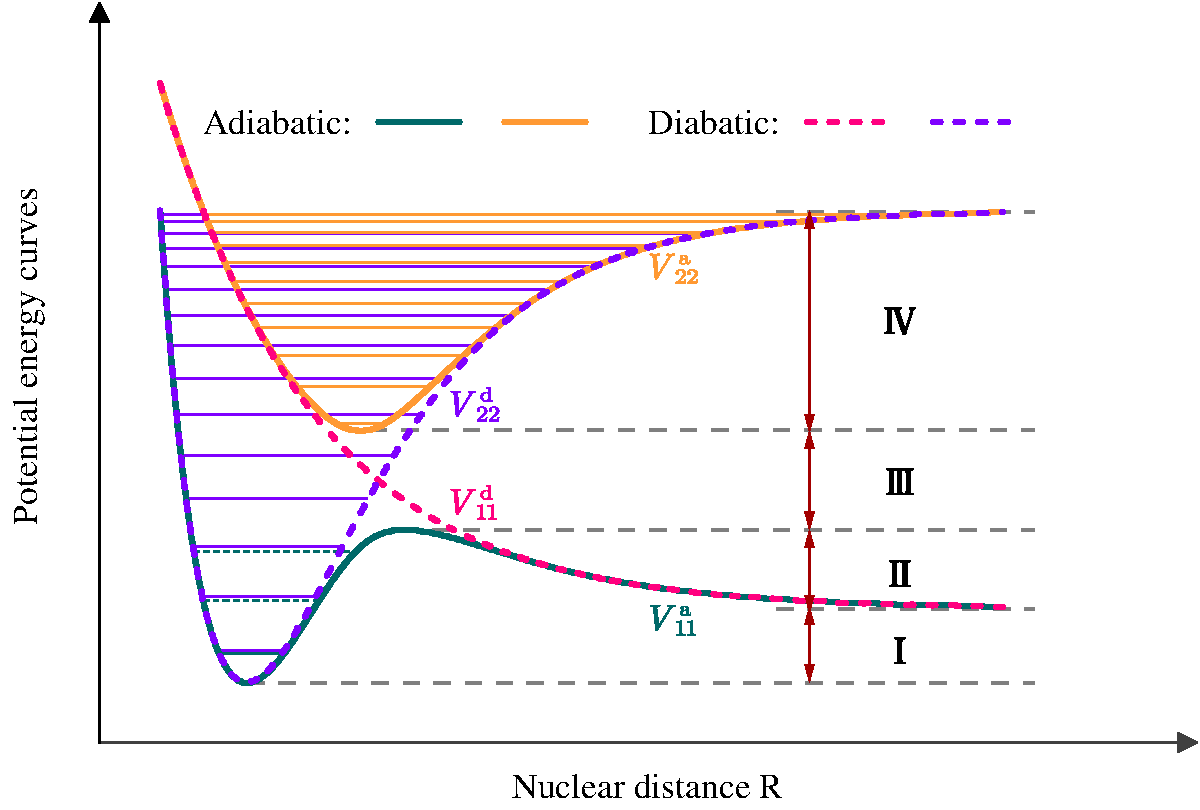
\includegraphics[width=0.5\linewidth]{pic/njpFigure1.pdf}
    \bicaption{绝热和非绝热表示中的典型势能曲线}{Typical potential energy curves in the adiabatic and diabatic representations}
    \label{fig:example}
\end{figure}


\section{进阶拼图}


\begin{figure}[!htbp]
    \centering
    \subfloat[势形共振]{\label{fig:shape}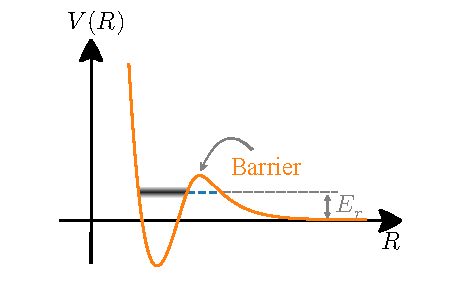
\includegraphics[width=.45\textwidth]{pic/Intro-pic_shape1.pdf}} \qquad
    \subfloat[Feshbach共振]{\label{fig:feshbach}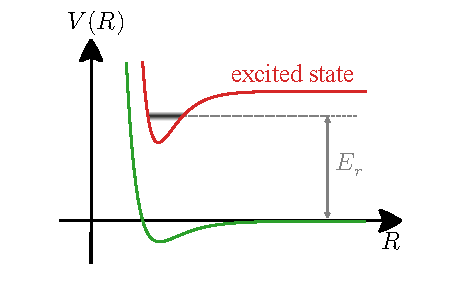
\includegraphics[width=.45\textwidth]{pic/Intro-pic_feshbach1.pdf}}
    \bicaption[势形共振和Feshbach共振示意图]{势形共振和Feshbach共振示意图}{Schematic for shape and Feshbach resonance}
    \label{fig:shapeandfeshbach}
\end{figure}     %% 第三章
            % -*- coding: utf-8 -*-
% !TEX program = xelatex


\chapter{表格的使用}



\section{简单三线表格}



\begin{table}[!htbp]
    \centering
    \bicaption{Child-Lefebvre 模型$ V_{22}^{\mathrm{d}} $势能曲线束缚态能量}{Bound energy for $ V_{22}^{\mathrm{d}} $ of Child-Lefebvre model}
    \scalebox{0.9}{    
    \begin{tabular}{cccccccc}
            \toprule
            \multicolumn{1}{c}{$\nu$} &\multicolumn{1}{c}{Bound of $ V_{22}^{\mathrm{d}} $} &\multicolumn{1}{c}{$\nu$} & \multicolumn{1}{c}{Bound of $ V_{22}^{\mathrm{d}} $}&\multicolumn{1}{c}{$\nu$} & \multicolumn{1}{c}{Bound of $ V_{22}^{\mathrm{d}} $}&\multicolumn{1}{c}{$\nu$} & \multicolumn{1}{c}{Bound of $ V_{22}^{\mathrm{d}} $}\\
            \cmidrule(r){1-2} \cmidrule(r){3-4} \cmidrule(r){5-6} \cmidrule(r){7-8}
            %\midrule
            0  & $0.0015853$ & 9  & $0.0269396$ & 18 & $0.0462668$ & 27 & $0.0595669$ \\
            1  & $0.0047001$ & 10 & $0.0293847$ & 19 & $0.0480422$ & 28 & $0.0606726$ \\
            2  & $0.0077404$ & 11 & $0.0317554$ & 20 & $0.0497432$ & 29 & $0.0617040$ \\
            3  & $0.0107064$ & 12 & $0.0340517$ & 21 & $0.0513698$ & 30 & $0.0626609$ \\
            4  & $0.0135980$ & 13 & $0.0362735$ & 22 & $0.0529220$ & 31 & $0.0635434$ \\
            5  & $0.0164151$ & 14 & $0.0384210$ & 23 & $0.0543998$ & 32 & $0.0643515$ \\
            6  & $0.0191578$ & 15 & $0.0404941$ & 24 & $0.0558032$ & 33 & $0.0650852$ \\
            7  & $0.0218262$ & 16 & $0.0424927$ & 25 & $0.0571322$ & 34 & $0.0657445$ \\
            8  & $0.0244201$ & 17 & $0.0444170$ & 26 & $0.0583867$ & 35 & $0.0663294$ \\
            \bottomrule
        \end{tabular}%
    }
\label{tab:ykchildmodelv22bound}
\end{table}%


\section{进阶旋转缩放表格}




%=========================================%
\begin{sidewaystable}[!htbp]
    \centering
    \bicaption{H$_{2}$-Ar系统Lennard-Jones势$\ell=7$分波共振参数}{Resonance parameters for Lennard-Jones potential $\ell=7$ in H$_{2}$-Ar system.}
    \scalebox{0.98}{
        \begin{tabular}{ccccccc}
            \toprule
            Methods & \multicolumn{2}{c}{Nicolaides~\emph{et al.}, ECS\cite{RN1271}} & \multicolumn{2}{c}{Connor~\emph{et al.}, CSM\cite{RN1273}}   & \multicolumn{2}{c}{Present CDM} \\
            \cmidrule(r){1-1} \cmidrule(r){2-3} \cmidrule(r){4-5} \cmidrule(r){6-7}
            State & $ E_{\ell=7}~(\text{a.u.})$ &  $ \Gamma_{\ell=7}~(\text{a.u.}) $ & $ E_{\ell=7}~(\text{a.u.})$ &  $ \Gamma_{\ell=7}~(\text{a.u.}) $ & $ E_{\ell=7}~(\text{a.u.})$ &  $ \Gamma_{\ell=7}~(\text{a.u.}) $\\
            \cmidrule(r){1-1} \cmidrule(r){2-2} \cmidrule(r){3-3} \cmidrule(r){4-4} \cmidrule(r){5-5} \cmidrule(r){6-6} \cmidrule(r){7-7}
            $D_{\text{e}}=40~\text{cm}^{-1}$ & $  4.99465\times 10^{-5}$ & $1.11721\times 10^{-5 } $ & $5.00103\times 10^{-5}$ & $1.13134\times 10^{-5 }$  &$4.99944\times 10^{-5}$ & $ 1.12902\times 10^{-5 }$\\
            $D_{\text{e}}=45~\text{cm}^{-1}$ & $  4.13396\times 10^{-5}$ & $4.68847\times 10^{-6 } $ & $4.13305\times 10^{-5}$ & $4.72036\times 10^{-6 }$  &$4.13146\times 10^{-5}$ & $ 4.71076\times 10^{-6 }$\\
            $D_{\text{e}}=50~\text{cm}^{-1}$ & $  3.18078\times 10^{-5}$ & $1.18784\times 10^{-6 } $ & $3.18032\times 10^{-5}$ & $1.18647\times 10^{-6 }$  &$3.17882\times 10^{-5}$ & $ 1.18265\times 10^{-6 }$\\
            $D_{\text{e}}=55~\text{cm}^{-1}$ & $  2.10047\times 10^{-5}$ & $9.04888\times 10^{-8 } $ & $2.10047\times 10^{-5}$ & $9.04888\times 10^{-8 }$  &$2.09882\times 10^{-5}$ & $ 9.00267\times 10^{-8 }$\\
            $D_{\text{e}}=60~\text{cm}^{-1}$ & $  8.78917\times 10^{-6}$ & $1.93872\times 10^{-10} $ & $8.78917\times 10^{-6}$ & $2.00980\times 10^{-10}$  &$8.77337\times 10^{-6}$ & $ 1.98465\times 10^{-10}$\\
            \toprule
        \end{tabular}%
    }
    \label{tab:j=7}%

\end{sidewaystable}












     %% 第四章
            % -*- coding: utf-8 -*-
% !TEX program = xelatex

\chapter{罗列环境的使用}



\section{普通罗列环境}



\begin{itemize}
    \addtolength{\itemsep}{-.36\baselineskip}%缩小条目之间的间距,下面类似
    \item 大漠孤烟直
    \item 长河落日圆
\end{itemize}




\begin{enumerate}
    \item 从散射理论出发。
    \item 从将共振态视为复哈密顿量本征值出发。
    \item 从共振态与呈指数衰减的波函数有关的观点出发(含时理论)。
\end{enumerate}

\section{进阶罗列环境}


\begin{yklist}{Feshbach共振}
    \item[势形共振] 势形共振是指隧穿势垒的共振,通常特指发生在单个通道。势能曲线有两个极点:一个极小点(平衡点),一个极大点(势垒)。形成这个势垒的原因有多种。例如,高分波离心势项$\frac{\hbar \ell(\ell+1)}{2\mu R^2}$ 会使有效势$ V_{\text{eff}}(R,\ell) $ 在较大核间距处出现一个离心势垒。
    \item[Feshbach共振] Feshbach共振又称成为Fano共振,或者Fano-Feshbach共振,是以物理学家H.~Feshbach和U.~Fano的名字命名\cite{RN1793,RN417,RN38},但是E.~Majorana才是第一个观测到这种现象的人\cite{RN2608}。
\end{yklist}










     %% 第五章
            % -*- coding: utf-8 -*-
% !TEX program = xelatex


\chapter{总结与展望}


     %% 总结与展望
        \sloppy                       %% 防止参考文献溢出
        \printbibliography[title=参考文献,heading=bibintoc]
        \phantomsection
        \begin{appendix}
            % -*- coding: utf-8 -*-
% !TEX program = xelatex


\chapter{附录}
\label{cha:auunit}



这里是附录。








     %% 原子单位
        \end{appendix}
    \backmatter
            % -*- coding: utf-8 -*-
% !TEX program = xelatex

\chapter{致谢}


致谢通常控制在一页以内。


\vskip 1.0cm

\begin{flushright}
    \begin{tabular}{c}
        {\zihao{-4}  杨玉坤} \\
        {\zihao{-4}  二〇二二年三月十九日}
    \end{tabular}
\end{flushright}
     %% 致谢
            % -*- coding: utf-8 -*-
% !TEX program = xelatex

\chapter{攻读博士学位期间研究成果}


\section*{第一作者发表论文} % 发表的和录用的合在一起




\begin{enumerate}[label = {[\arabic*]}]
    \addtolength{\itemsep}{-.36\baselineskip}%缩小条目之间的间距,下面类似
    \item \textbf{Y. K. Yang} and S. B. Zhang, “XXX XXX XXX”
    \textit{XXX}, 11, 11111 (2022).
    \item \textbf{Y. K. Yang} and S. B. Zhang, “XXX XXX XXX”
    \textit{XXX}, 11, 11111 (2021).
    \item \textbf{Y. K. Yang} and S. B. Zhang, “XXX XXX XXX”
    \textit{XXX}, 11, 11111 (2020).
    \item \textbf{Y. K. Yang} and S. B. Zhang, “XXX XXX XXX”
    \textit{XXX}, 11, 11111 (2019).
\end{enumerate}








\section*{获奖情况} % 参加项目

\begin{enumerate}[label = {[\arabic*]}]
    \addtolength{\itemsep}{-.36\baselineskip}%缩小条目之间的间距,下面类似
    \item 2021 年 12 月,陕西师范大学博士一等积学奖学金 \par
    \item 2020 年 12 月,陕西师范大学博士二等积学奖学金 \par
    \item 2019 年 12 月,陕西师范大学博士一等积学奖学金 \par
    \item 2019 年 08 月,第二十届全国原子与分子物理学术会议优秀海报奖 \par
\end{enumerate}







\section*{参与学术会议情况} % 参加项目




\begin{enumerate}[label = {[\arabic*]}]
    \addtolength{\itemsep}{-.36\baselineskip}%缩小条目之间的间距,下面类似
    \item 2021 年 09 月 24 日  —— 2021 年 09 月 27 日 \\ 第二十一届全国原子与分子物理学术会议·大连 \quad 口头报告 \& 墙报报告
    \item 2019 年 08 月 16 日  —— 2019 年 08 月 20 日 \\ 第二十届全国原子与分子物理学术会议·洛阳 \quad 墙报报告
    \item 2019 年 07 月 07 日  —— 2019 年 07 月 12 日 \\ 2019年清华大学低维量子物理国家重点实验室暑期学校·北京 
    \item ……
\end{enumerate}
























% \begin{enumerate}[label = {[\arabic*]}]
%     \addtolength{\itemsep}{-.36\baselineskip}%缩小条目之间的间距,下面类似
%     \item 2021 年 09 月 24 日,大连,第二十一届全国原子与分子物理学术会议。\\墙报报告 \& 口头报告 
%     \item 2019 年 08 月 16 日,洛阳,第二十届全国原子与分子物理学术会议。\\墙报报告 
%     \item 2019 年 07 月 07 日,北京,2019年清华大学低维量子物理国家重点实验室暑期学校 
%     \item 2019 年 05 月 17 日,绵阳,第三届原子分子光物理学术研讨会
%     \item 2019 年 03 月 24 日,西安,第三届复杂系统论坛%:x-ray in AMO and related topics 
%     \item 2019 年 01 月 25 日,西安,等离子体中原子物理问题研讨会
%     \item 2018 年 08 月 06 日,临汾,第七届全国计算原子与分子物理学术会议 。\\墙报报告
%     \item 2018 年 05 月 18 日,西安,第三届原子分子光物理学术研讨会 
%     \item 2017 年 10 月 12 日,西安,第四届原子分子精密谱研讨会 
%     \item 2017 年 08 月 06 日,长春,第十九届全国原子与分子物理学术会议 
%     \item 2017 年 05 月 13 日,北京,第二届原子分子光物理学术研讨会  
% \end{enumerate}



     %% 研究成果
\end{document}



